We are now concerned with the example 8.1 and we will try different methods to solve it.
\subsection*{a) Upwind method} 

We are first going to use the upwind method to solve the problem. The first step is to discretize the equation. The PDE is :

$$\frac{\dr T}{\dr t}+v\frac{\dr T}{\dr x}+ a(T-T_{cool})=0$$

Using forward time and backward space differences and denoting $T_{i,k} \approx T(ih_x,kh_t)$, we get :

\begin{align*}
&\frac{T_{i,k+1}-T_{i,k}}{h_t}+v\frac{T_{i,k}-T_{i-1,k}}{h_x}+a(T_{i,k}-T_{cool})=0\\
&T_{i,k+1} = (1-\frac{vh_t}{hx}-ah_t)T_{i,k}+\frac{vh_t}{h_x}T_{i-1,k}+ah_tT_{cool}
\end{align*}

Because we have an initial condition and a boundary condition for $x=0$, we problem is well posed. The implementation is done in the code $temp.m$. Figure \ref{up} presents the results for the implementation of the upwind method for the given problem.

\begin{figure}
\begin{center}
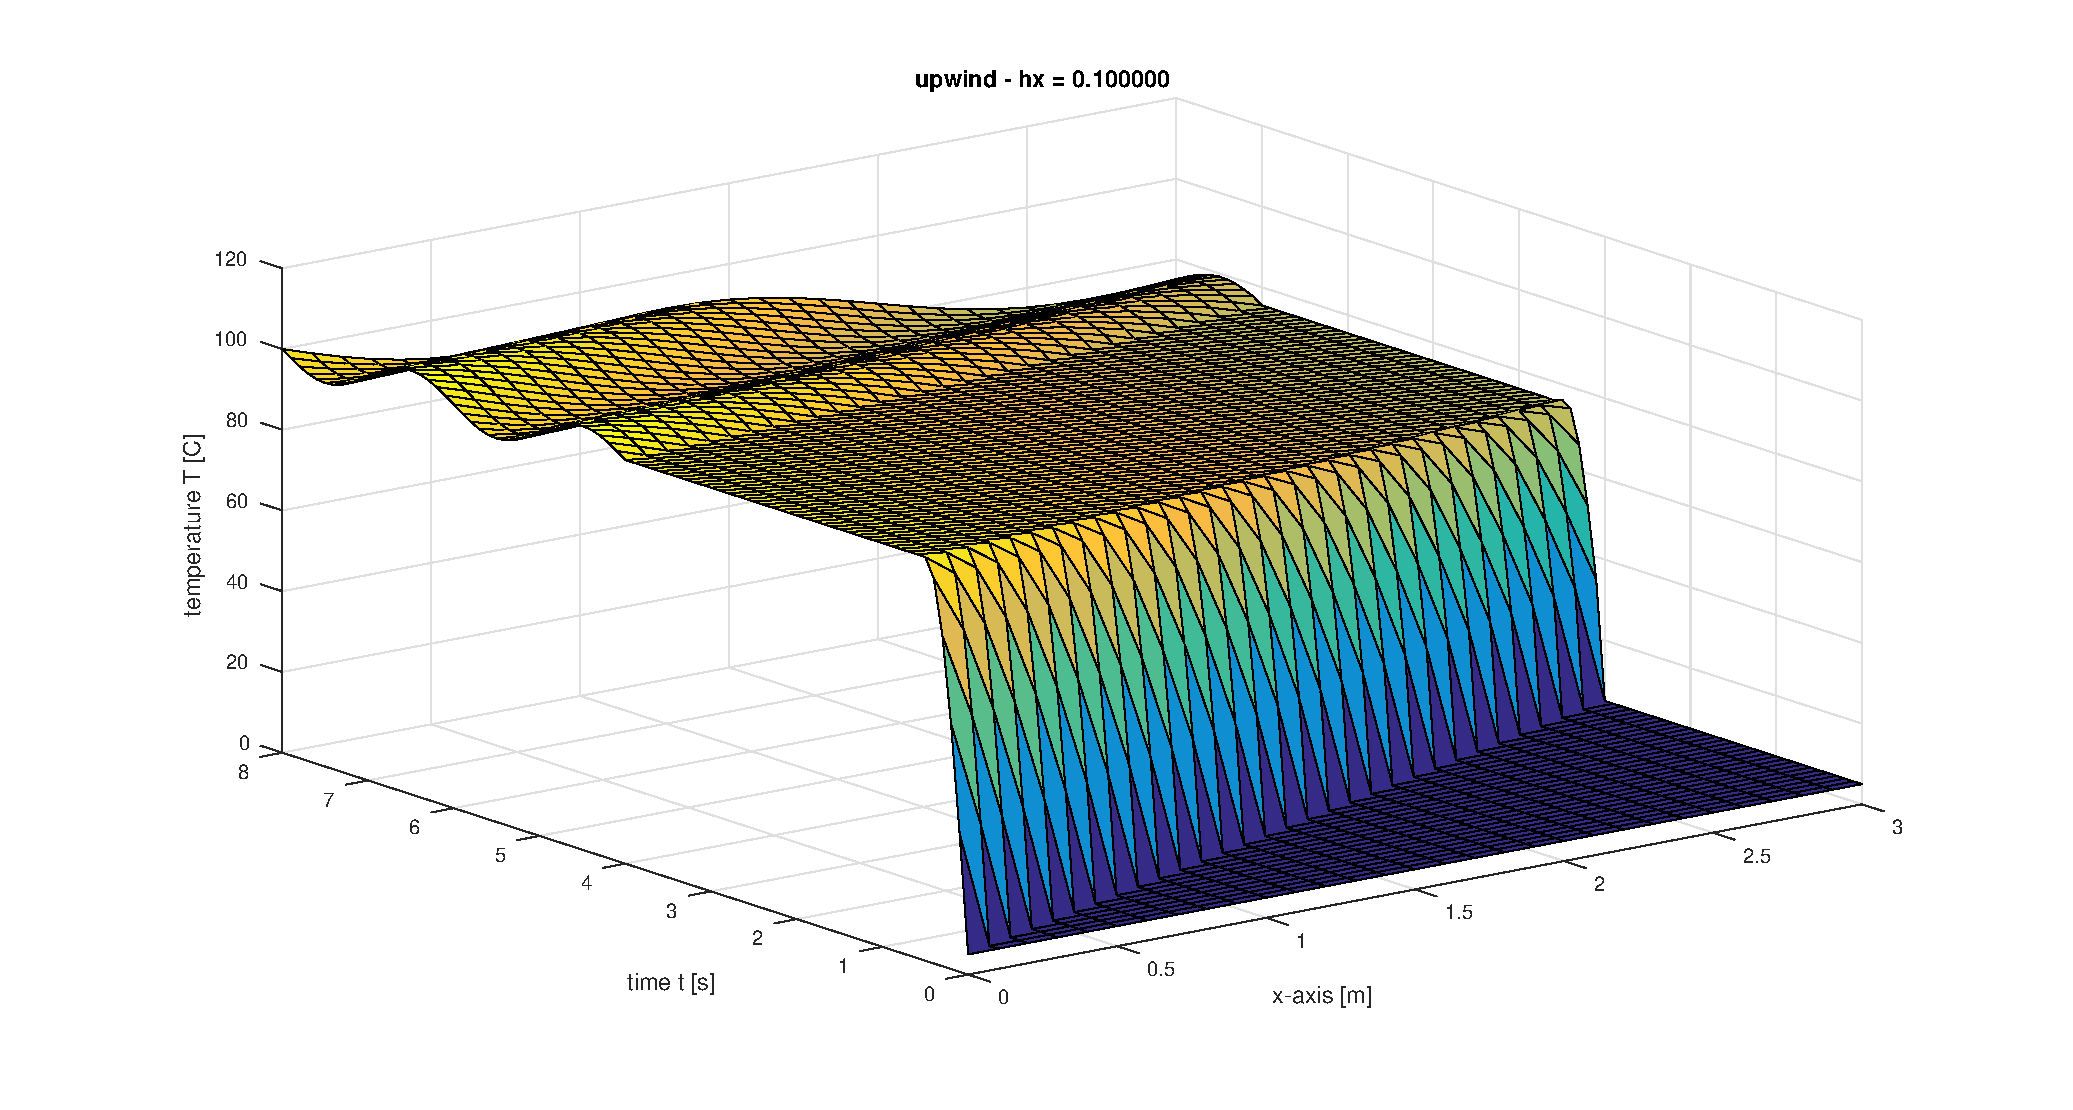
\includegraphics[scale=0.4]{upwind.eps}
\caption{Solution with upwind method}
\label{up}
\end{center}
\end{figure}

The figure presents what is to be expected. At $x=0$, we can see the given boundary condition. We also see that the temperature propagates along the x-axis but that there are some dissipation and that the mean temperature decreases as we go along the x-axis.

\subsection*{b) Derivation of the Lax-Wendroff rule}
In this part, we are going to try to compute a Lax-Wendroff rule for the problem. The trick is to use the PDE to express the time derivatives with spacial derivatives and then use Taylor expansion. So, in this instance, we have :

$$\frac{\dr T}{\dr t}=-v\frac{\dr T}{\dr x}-a(T-T_{cool})$$

So the second order derivative, we have :
\begin{align*}
\frac{\dr^2T}{\dr t^2} &= \frac{\dr}{\dr t}( -v\frac{\dr T}{\dr x}-a(T-T_{cool}))\\
&=-v\frac{\dr}{\dr x}(\frac{\dr T}{\dr t})-a\frac{\dr T}{\dr t}\\
&=-v\frac{\dr}{\dr x}(-v\frac{\dr T}{\dr x}-a(T-T_{cool})) - a(-v\frac{\dr T}{\dr x}-a(T-T_{cool}))\\
&=v^2\frac{\dr^2 T}{\dr x^2}+2av\frac{\dr T}{\dr x}+a^2(T-T_{cool})
\end{align*}

Now we use Taylor expansion up until the second order : 
\begin{align*}
T_{i,k+1} &= T_{i,k}+h_t \frac{\dr T}{\dr t}+\frac{h_t^2}{2}\frac{\dr^2 T}{\dr t^2}\\
&=T_{i,k}+h_t(-v\frac{\dr T}{\dr x}-a(T-T_{cool}))+\frac{h_t^2}{2}(v^2\frac{\dr^2 T}{\dr x^2}+2av\frac{\dr T}{\dr x}+a^2(T-T_{cool})) 
\end{align*}

Using central differences for spatial derivatives, we get : 
$$T_{i,k+1} = c_1T_{i-1,k}+c_2T_{i,k}+c_3T_{i+1,k}+c_4$$

Where the $c_i$ are defined by : 
\begin{align*}
c_1 &= \frac{h_tv}{2h_x}+\frac{h_t^2v^2}{2h_x^2}-\frac{avh_t^2}{2h_x}\\
c_2 &=1-ah_t+\frac{a^2h_t^2}{2}-\frac{v^2h_t^2}{h_x^2}\\
c_3 &= -\frac{vh_t}{2h_x}+\frac{v^2h_t^2}{2h^2}+\frac{avh_t^2}{2h_x}\\
c_4 &= (ah_t - \frac{a^2h_t^2}{2})T_{cool}
\end{align*}

\subsection*{c) Presentation of the results}
In this final part, we are going to use the Lax-Wendroff formula derived in the previous part. We have first to notice that because we need both the point to the right and the point to the left, we will have to use the extrapolation formula already used in the first part for the right end point (that is for $x=L$). That is : 
$$T_{end,k} = 2T_{end-1,k}-T_{end-2,k}$$

Using this and the boundary condition given, we can implement the problem. This is also done in $temp.m$. Figure \ref{lw} presents the results. 

\begin{figure}
\begin{center}
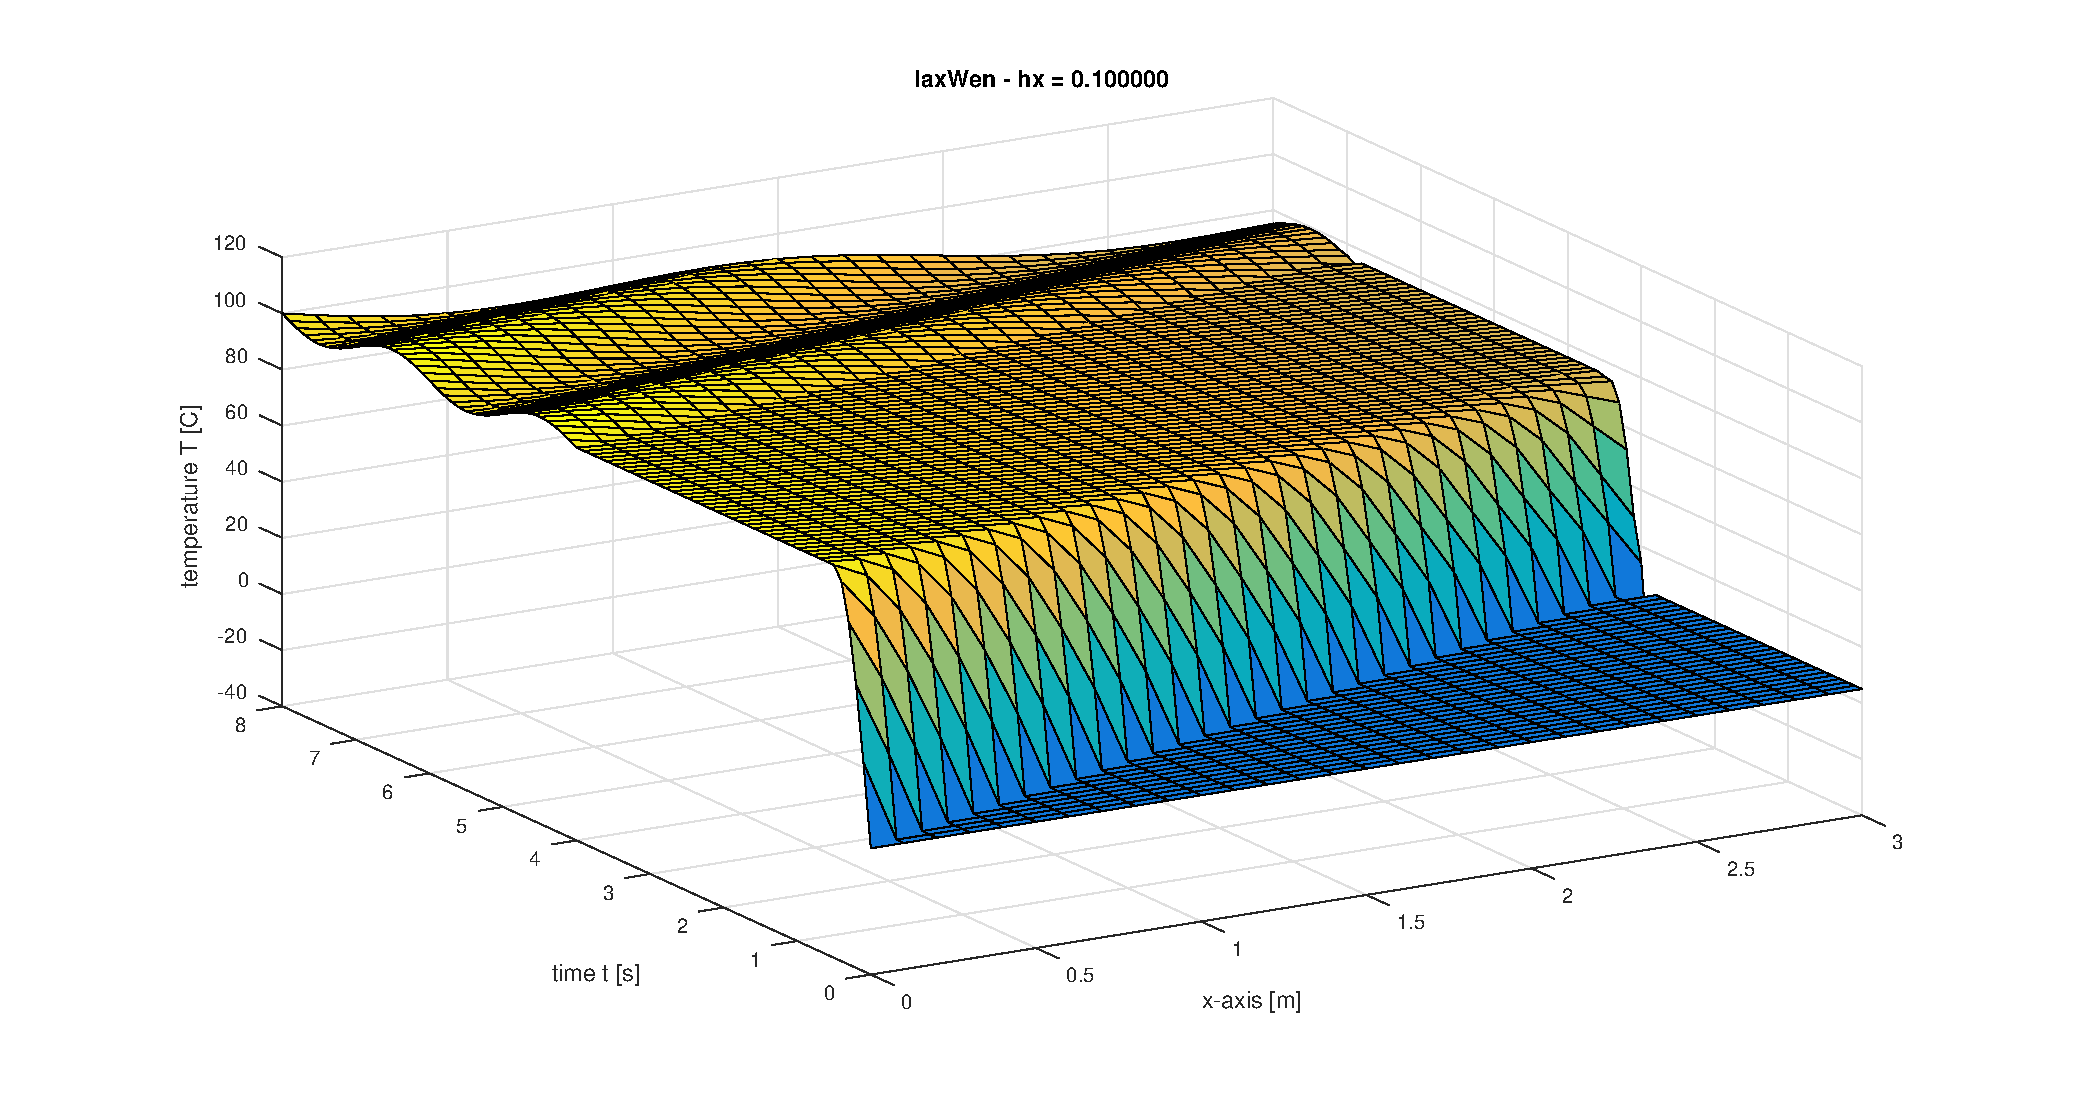
\includegraphics[scale=0.4]{laxWen.eps}
\caption{Solution with Lax-Wendroff method}
\label{lw}
\end{center}
\end{figure}

We can see that this plot is very similar to the one obtained with the upwind method. All the remarks done previously thus hold. The only notable difference is that we can see a peak due to the extrapolation formula on the far right end side (as shown on figure \ref{trois}).

\begin{figure}
\begin{center}
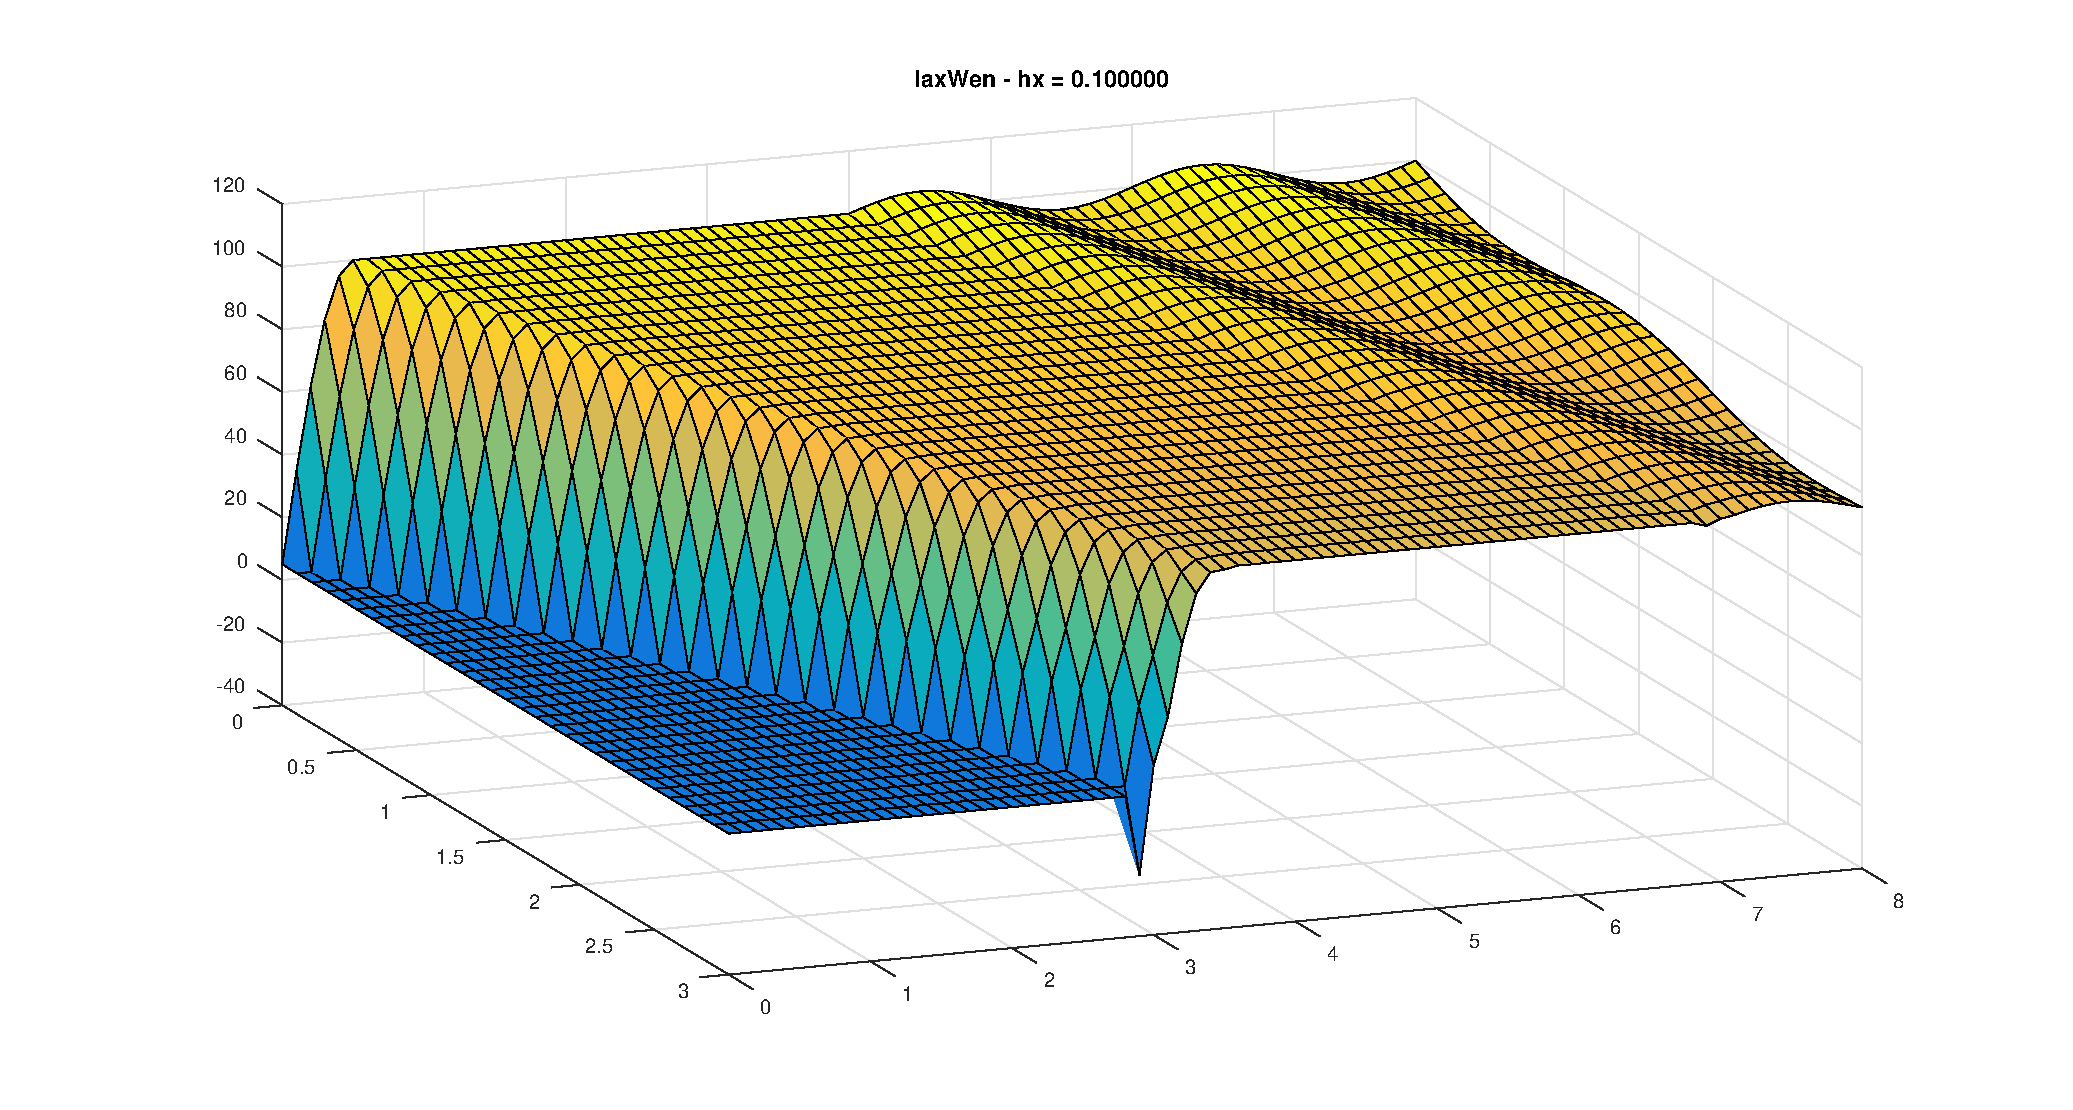
\includegraphics[scale=0.4]{fig3.eps}
\caption{Oscillation due to extrapolation}
\label{trois}
\end{center}
\end{figure}

\FloatBarrier

\section*{Matlab codes}

\lstinputlisting{transport.m}
\lstinputlisting{temp.m}